\documentclass[a4paper,12pt]{article}
%\documentclass[letterpaper,11pt]{article}
 \setlength{\parskip}{0pc}
 \setlength{\textwidth}{38pc}
 \setlength{\textheight}{56pc} 
 \setlength{\topmargin}{-1.2cm}
 \setlength\oddsidemargin{0cm}  
 \setlength\evensidemargin{0cm} 

\usepackage{setspace}

\usepackage{latexsym} % yw acrescentou

\usepackage[utf8]{inputenc}
\usepackage[english]{babel}

\usepackage{amsfonts,amsmath,amssymb,amsbsy,amsthm,enumerate}
%\usepackage{graphics,graphicx,subfigure,psfrag}

\usepackage[mathscr]{euscript}
%\usepackage{bbm}
%\usepackage{authblk}
%\usepackage{arydshln}
\usepackage{pstricks}
\usepackage{multirow}
\usepackage{verbatim}
\usepackage{color}

\sloppy

\newtheorem{theorem}{Theorem}[section]
\newtheorem{lemma}{Lemma}[section]
\newtheorem{claim}{Claim}


\newcommand{\imm}{\subseteq_{IM}}

\bibliographystyle{plain}

%%TIKZ
\usepackage{tikz}
\usepackage[subrefformat=parens,labelformat=parens]{subcaption}
\usetikzlibrary{calc,positioning,decorations.pathmorphing,decorations.pathreplacing}
\tikzset{black vertex/.style={circle,draw,minimum size=1mm,inner sep=0pt,outer sep=2pt,fill=black, color=black}}
%\tikzset{largepath/.style={orange!75!white,line width=6pt,line cap=round,opacity=0.5}}

%\usepackage{graphicx}

\title{Immersions of cliques in graphs \\ with bounded maximum degree}

\begin{document}

\maketitle

\section{Andrasfai graphs and its relatives}

Andrasfai graphs are well-known triangle-free graphs. 
Any blow-up of an Andrasfai graph is also triangle-free.
So the complement of these graphs have independence number at most 2. 
In what follows we study immersions of cliques in this class of graphs. 
 
Let \(k\) be a positive integer, and let \(F_k\) be the Andrasfai graph of order $k$.
Note that \(h = v(F_k) = 3k-1\) and \(\omega(F_k) = k\).
Let \(G\) be a graph such that \(\overline{G}\) is a blow-up of \(F_k\), 
and let \(V_1,\ldots, V_h\) be the blow-up vertex classes.
Say \(G\) has \(n\) vertices.
Let \(K\) be a maximum clique in \(G\).
One can prove that \(V(K)\) is the disjoint union of precisely \(k\) of the blow-up vertex classes.
Moreover we may assume without loss of generality that \(V(K) = \cup_{i=0}^{k-1} V_{3i+1}\).
In what follows, we find an immersion in \(G\) of a clique in which the branch vertices are 
precisely \(V(G)\setminus V(K)\).

Let \(I = \{2,3,5,6,\ldots,3k-4,3k-3\}\) be the indices of the blow-up vertex classes
corresponding to \(V(G)\setminus V(K)\).
We say a family \(\{A_i: i \in I\}\) of subsets of \(V(K)\) is a \emph{helpful set family} 
if it satisfies the following conditions for every \(i \in I\):
\begin{enumerate}
\item \(|A_i| = |V_i|\);
\item \(A_i \subseteq \overline{N_G(V_i)} \cap V(K)\);
\item the sets \(A_j\) with \(j \in N_{F_k}[i]\cap I\) are mutually disjoint, 
  that is, if \(j,j' \in N_{F_k}[i] \cap I\), then \(A_j\cap A_{j'} = \emptyset\).
\end{enumerate}

\begin{lemma}
  If \(G\) has a helpful set family, then there is an immersion in \(G\) of 
  a clique in which the branch vertices are precisely \(V(G)\setminus V(K)\).
\end{lemma}

\begin{lemma}
  Graph \(G\) has a helpful set family. 
\end{lemma}

This implies the following: 

\begin{theorem}
 The vertex set of the complement of any blow up of an Andrasfai graph can be partitioned 
 into a clique and the branch vertices of an immersion of a clique. 
\end{theorem}


\section{Graphs whose complements admit a special \(3\)-coloring}

\newcommand{\Gcompl}{\overline{G}}

Given a positive integer \(k\),
a \emph{\(k\)-clique-coloring} of a graph \(G\) is a partition \(\{C_1,\ldots, C_k\}\) of \(V(G)\)
such that \(C_i\) is a clique of \(G\) for every \(i\in[k]\).

\begin{theorem}
	Let \(G\) be a graph with \(\alpha(G) = 2\)
	and that admits a \(3\)-clique coloring \(\{C_1,C_2,C_3\}\) such that
	(i) \(C_1\) is a maximum clique of \(G\); and
	(ii) \(G[C_2\cup C_3]\) has no induced \(C_4\).
	Then \(G\) contains an immersion of a clique whose set of branch vertices is precisely \(C_2\cup C_3\).
\end{theorem}

\begin{proof}
	Observe that \(C_1,C_2,C_3\) is a \(3\)-coloring of \(\Gcompl\),
	and by hypothesis \(C_1\) is a maximum independent set of \(\Gcompl\).
	Let \(i\in\{2,3\}\) and let \(C\subseteq C_i\).
	If \(|N_{C_1}(C)| < |C|\), 
	then \((C_1\setminus N_{C_1}(C))\cup C\) is an independent set that is larger than \(C_1\),
	a contradiction to the maximality of \(C_1\).
	Then \(|N_{C_1}(C)| \geq |C|\) for any subset of \(C_i\).
	By Hall's Theorem, there is a matching \(M_i\) in \(\Gcompl[C_i,C_1]\) that covers \(C_i\).
	
	Given a vertex \(u\in C_2 \cup C_3\), 
	note that there is precisely one edge in \(M_2\cup M_3\) that contains \(u\),
	and let \(r_u\in C_1\) be the vertex such that \(ur_u\in M_2\cup M_3\).
%	We say that \(r_u\) is the \emph{representative} of \(u\).
	Note that \(r_u \notin N(u)\),
	and hence, since \(\alpha(G) = 2\), \(r_u\) is adjacent to every vertex in \(V(G)\setminus N[u]\).
	In what follows, let \(E' = E\big(G[C_2,C_3]\big)\).
	Note that if \(u\in C_2\) and \(v\in C_3\) are such that \(r_u = r_v = w\),
	then \(uv \in E'\), otherwise \(u,v,w\) would be an independent set of size \(3\).
%	
	Note that if \(uv\notin E'\) we have \(r_u\in N(v)\), \(r_v\in N(u)\),
	and since \(C_1\) is a clique, \(r_ur_v\in E(G)\).

	Now, for every \(uv\notin E'\), let \(P_{uv}\) be the path \(u r_v r_u v\).
	We claim that the paths \(P_e\) with \(e\notin E'\) are pairwise edge-disjoint.
	Indeed, let \(u,u' \in C_2\) and \(v,v' \in C_3\) be such that \(uv,u'v' \notin E'\)
	and \(uv \neq u'v'\).
	Note that \(u\) and \(u'\) (resp. \(v\) and \(v'\)) are not necessarily distinct,
	but either \(u \neq u'\) or \(v \neq v'\).
	If \(v\neq v'\), then \(r_v \neq r_{v'}\) because \(M_3\) is a matching.
	This implies that \(ur_v \neq u'r_{v'}\) (even if \(u = u'\)).
	Analogously, we have \(vr_u \neq v'r_{u'}\).
	In what follows, we prove that \(r_ur_v \neq r_{u'}r_{v'}\).
	Suppose, for a contradiction, that \(r_ur_v = r_{u'}r_{v'}\).
	If \(r_u = r_{u'}\) and \(r_v = r_{v'}\), then \(u=u'\) and \(v=v'\), a contradiction.
	Thus, we may assume \(r_u = r_{v'}\) and \(r_v = r_{u'}\).
	As noted above, this implies that \(uv',vu' \in E'\) (see Figure~\ref{fig:induced-C4}).
	But then \(\{u,v,u',v'\}\) induce a \(C_4\) in \(G[C_2\cup C_3]\),
	a contradiction .
\end{proof}

\begin{figure}[ht]
    \centering
        \centering
        \begin{tikzpicture}[scale = 0.8]
        
        \node (u)	[black vertex] at	(-2,-1)	{};
        \node (u')	[black vertex] at	(-2,1)	{};
        \node (v)	[black vertex] at	(2,-1)	{};
        \node (v')	[black vertex] at	(2,1)	{};
        \node (ru)	[black vertex] at	(1,3)	{};
        \node (rv)	[black vertex] at	(-1,3)	{};
        
        \node [anchor=north]		at		(u)		{$u$};
        \node [anchor=south east]	at		(u')	{$u'$};
        \node [anchor=north]		at		(v)		{$v$};
        \node [anchor=south west]	at		(v')	{$v'$};
        \node [anchor=north]		at		(ru)	{$r_u$};
        \node [anchor=north]		at		(rv)	{$r_v$};
        \node [anchor=south east]	at		(ru)	{$r_{v'}$};
        \node [anchor=south west]	at		(rv)	{$r_{u'}$};

        
        \draw [thick] (u) -- (u') (v) -- (v') (ru) -- (rv);
        \draw [thick] (ru) to [bend left = 90] (v) (ru) -- (u');
        \draw [thick] (rv) to [bend right = 90] (u) (rv) -- (v');
        \draw [thick,dashed] (u) -- (v) (u') -- (v');
        \draw [thick] (u) -- (v') (v) -- (u');
        \draw [thick,dashed] (u) to [bend left = 15] (ru) (v) to [bend right = 15] (rv) (u') to [bend left] (rv) (v') to [bend right] (ru);
        \end{tikzpicture}
    \caption{}
    \label{fig:induced-C4}
\end{figure}

\section{An alternative proof of the existence of immersions of $K_{2n/5}$}




\begin{theorem}
    Let \(G\) be a graph on \(n\) vertices.
    If $\alpha(G)\leq 2$, then $K_{2\lfloor n/5\rfloor}\imm G$.
\end{theorem}
\begin{proof}
    The proof follows by induction on \(n(G) + e(G)\).
    One can easily check that the statement holds for \(n\leq 5\).
    Since we seek an immersion with only $2\lfloor n/5\rfloor$ vertices, we may also assume $n=5t$ for some $t\geq2$, and thus \(n\geq 10\).

    Let \(G\) be a graph on \(n\) vertices for which \(\alpha(G) \leq 2\).
    If \(\alpha(G-e) \leq 2\) for some edge \(e\in E(G)\),
    then, by the induction hypothesis, \(K_{2n/5} \imm G-e \subseteq G\), as desired.
    Therefore, we can assume that \(G\) is minimal with \(\alpha(G) \leq 2\).
    Moreover, the minimality implies \(\alpha(G) = 2\),
    and, in particular, \(G\) is not a complete graph.

    Also,
    since $\alpha(G)\leq 2$, 
    the set $\overline{N(u)} = V(G)\setminus N(u)$ induces a clique for every $u\in V(G)$.
    Thus, if \(|\overline{N(u)}| \geq 2n/5\) for some vertex \(u\in V(G)\),
    then \(\overline{N(u)}\) induces the desired immersion.
    Therefore, we may assume that \(|\overline{N(u)}| < 2n/5\)
    for every \(u\in V(G)\).
    This implies that \(|N(u)| \geq 3n/5\) for every \(u\in V(G)\).
    
    % If \(G\) is a complete graph, then $K_{n}\subseteq G$,
    % and hence \(G\) has the desired immersion.
    % Thus, we may assume that \(G\) is not a complete graph.


    % We will show that such immersion exists by induction.
    % Let $G$ be a counterexample to the claim, and minimal in vertices.
   
\begin{claim}
    %TODO: Transformar isso aqui em proposição, um G minimal...
    \(G\) has an induced copy of \(C_5\)
\end{claim}
\begin{proof}
    First, we claim that \(G\) contains an induced path of length \(2\).
    % TODO: verificar na literatura se nonadjacent é junto ou com hífen
    Indeed,
    since \(G\) is not a complete graph, 
    there is at least a pair \(u\) and \(v\) of nonadjacent vertices.
    Let \(P\) be a shortest path joining \(u\) and \(v\).
    Then \(P\) must be an induced path, and since \(u\) and \(v\) are nonadjacent, \(P\) contains  an induced path of length \(2\) as desired.

    Let \(v_1v_2v_3 \subseteq G\) an induced path of length \(2\).
    By Lemma \ref{lem:edgedomination}, there is a vertex $v_4$ that is non-adjacent to both $v_1$ and $v_2$;
    and there is a vertex $v_5$ that is non-adjacent to both $v_2$ and $v_3$.
    Since \(v_1\) is nonadjacent to both \(v_3\) and \(v_4\),
    then \(v_3v_4\in E(G)\).
    Analogously, \(v_1v_5, v_4v_5\in E(G)\),
    and hence \(\{v_1,v_2,v_3,v_4,v_5\}\) induce a copy of \(C_5\)
    in \(G\) as desired.
%
    % Let $v_1v_2\in E(G)$. 
    % By Lemma \ref{lem:edgedomination}, there is a vertex $v_4$ that is non-adjacent to both $v_1$ and $v_2$.
    % Also from Lemma \ref{lem:edgedomination}, there are vertices which dominate the non-edges $v_1v_4\not\in E(G)$ and $v_2v_4\not\in E(G)$, which well call $v_5$ and $v_3$, respectively. 
    % Clearly, $\{v_1, v_2, v_3, v_4, v_5\}$ is a $C_5$.
\end{proof}

%   TODO: falar sobre branch vertices 

    Let \(C\) be an induced copy of \(C_5\) in \(G\),
    and assume that \(V(C) = \{v_1,v_2,v_3,v_4,v_5\}\).
    % We take a cycle with vertices $C=\{v_1, v_2, v_3, v_4, v_5\}$ in $G$.
    By the induction hypothesis, we have \(K_{2n/5 - 2} \imm G\setminus V(C)\).
    Let \(K'\) be such an immersion,
    and let \(I \subseteq V(G)\setminus V(C)\) be the branch vertices of \(K'\).

    \begin{claim}
        Every vertex in $V(G)\setminus V(C)$ is adjacent to three consecutive vertices in $C$.
    \end{claim}
    \begin{proof}
    Let \(u \in V(G)\setminus V(C)\).
    If $u$ is adjacent to every vertex of $C$, the statement follows.
    Suppose, without loss of generality, that $u$ is not adjacent to $v_1$. 
    Since $v_1v_3,v_1v_4\not\in E(C)$ and \(\alpha(G) \leq 2\),
    $u$ is adjacent to $v_3$ and $v_4$. 
    Now, since $v_2v_5\not\in E(C)$ and \(\alpha(G) \leq 2\), 
    \(u\) is either adjacent to \(v_2\) or to \(v_5\),
    as desired.
    \end{proof}

    Partition $V(G)\setminus(I\cup V(C))$ into five sets, $Z_1, \ldots, Z_5$ such that if $u\in Z_i$ then $v_{i-1},v_i,v_{i+1}\in N(u)$,
    where the addition in the subscript are taken modulo \(5\).
    Observe that a vertex \(u \notin V(C)\) may fit in more than one such \(Z_i\).
    When this is the case, we choose one such \(Z_i\) arbitrarily.
    Then \(|Z_1| + \cdots + |Z_5| = |V(G)\setminus(I\cup V(C))| = n - (2n/5 - 2 + 5) = 3(n-5)/5\), and hence there is $i$ for which
    \begin{equation}\label{eq:Zi}
        |Z_i|\leq\frac{3}{25}(n-5).
    \end{equation}

    We may assume, without loss of generality, that $|Z_2|\leq\frac{3}{25}(n-5)$.
    Now, for \(i \in\{1,3\}\), let 
    \[X_i = I\setminus N(v_i) \qquad\text{and}\qquad Y^+_i=N(v_i)\setminus(I\cup V(C)).\]
    Since $v_1v_3\not\in E(G)$, it follows that $Y^+_1\cup Y^+_3=V(G)\setminus(I\cup V(C))$,
    and $X_1\cap X_3 = \emptyset$.
    The next claim is an important step in this proof.
    
    \begin{claim}
    There are $Y_1\subseteq Y^+_1\setminus Z_2$ and $Y_3\subseteq Y^+_3\setminus Z_2$ such that  
    \begin{enumerate} %TODO: trocar números por letras
        \item $|Y_1|=|X_1|$ and $|Y_3|=|X_3|$
        \item $Y_1\cap Y_3 = \emptyset$    
    \end{enumerate}
    \end{claim}
    \begin{proof}
        Let \(i\in \{1,3\}\),
        and note that $N(v_i) = |Y^+_i|+|I\setminus X_i|+2$.
        Observe that \(|I\setminus X_i| = |I| - |X_i| = \frac{2}{5}(n-5) - |X_i|\), and hence
         \[
            |Y^+_i|+\frac{2}{5}(n-5)-|X_i|+2
            % = |Y^+_i|+|I|-|X_i|+2
            = |Y^+_i|+|I\setminus X_i|+2
            = |N(v_i)|
            \geq \frac{3n}{5}
        \]
        Therefore, we have
        \begin{equation}\label{eq:lowerbound:Yi+}
            |Y^+_i|\geq \frac{n}{5}+|X_i|.
        \end{equation}
        
        We choose $Y_1\subseteq Y^+_1\setminus Z_2$ with $|Y_1|=|X_1|$, 
        giving priority to vertices not in $Y^+_1\cap Y^+_3$.
        This choice implies that either $Y_1\subseteq Y^+_1\setminus Y^+_3$
        or $(Y^+_1\setminus Y^+_3)\subseteq Y_1$.
%       
        If $Y_1\subseteq Y^+_1\setminus Y^+_3$,
        then by \eqref{eq:Zi} and \eqref{eq:lowerbound:Yi+},
        we have $|Y^+_3\setminus Z_2| \geq \frac{n}{5} + |X_3|-\frac{3}{25}(n-5)\geq |X_3|$, and we can choose \(Y_3\) as desired.
%        
        On the other hand, if $(Y^+_1\setminus Y^+_3)\subseteq Y_1$, then 
        we have \(V(G) \setminus (I \cup V(C)) = Y_1^+ \cup Y_3^+ = Y_1 \cup (Y_3^+\setminus Y_1)\), and since \(Y_1 \cap (Y_3^+\setminus Y_1) = \emptyset\), 
        we have
        \begin{align*} %TODO: Verificar essa última conta
            |Y_3^+\setminus (Y_1\cup Z_2)| 
                \geq |Y_3^+\setminus Y_1| - |Z_2| 
                & = |V(G)\setminus(I\cup V(C))| - |Y_1| - |Z_2|\\
                & = |V(G)\setminus(I\cup V(C))|-|Z_2|-|X_1| \\
                &  \geq \frac{3}{5}(n-5)-\frac{3}{25}(n-5)-|X_1| \\
                &   >    \frac{3}{5}(n-5)-\frac{1}{5}(n-5)-\frac{2}{5}(n-5)+|X_3| 
                \geq |X_3|,
        \end{align*}
        where we used that \(|X_1| + |X_3| \leq \frac{2}{5}(n-5)\) 
        because \(X_1\) and \(X_3\) are disjoint sets in~\(I\).
        Therefore, we can choose \(Y_3\) as desired.
    \end{proof}

    \begin{figure}[h]
\label{fig:inductionfor2n/5}
\centering
\begin{tikzpicture}
%TODO: Corrigir o caminho e adicionar um outro caminho
% Clique with 5 vertices in the bottom left corner
\node[draw, circle, fill=black, inner sep=1pt, label=right:$v_3$] (c1) at (1cm, 0) {};
\node[draw, circle, fill=black, inner sep=1pt, label=above right:$v_2$] (c2) at (0.309cm, 0.951cm) {};
\node[draw, circle, fill=black, inner sep=1pt, label=above left:$v_1$] (c3) at (-0.809cm, 0.588cm) {};
\node[draw, circle, fill=black, inner sep=1pt, label=below left:$v_5$] (c4) at (-0.809cm, -0.588cm) {};
\node[draw, circle, fill=black, inner sep=1pt, label=below right:$v_4$] (c5) at (0.309cm, -0.951cm) {};

\draw (c1) -- (c2);
\draw (c1) -- (c3) [red, dotted];
\draw (c1) -- (c4) [red, dotted];
\draw (c1) -- (c5);
\draw (c2) -- (c3) node[midway, above left, font=\large] {C};
\draw (c2) -- (c4) [red, dotted];
\draw (c2) -- (c5) [red, dotted];
\draw (c3) -- (c4);
\draw (c3) -- (c5) [red, dotted];
\draw (c4) -- (c5);

% Ellipse divided in 3 parts on the upper left
\draw[draw] (0, 3) ellipse (1.5 and 0.7);
\draw (-0.7,2.38) -- (-0.7,3.62);
\draw (0.7,2.38) -- (0.7,3.62);
\node at (-1, 3.2) {$X_1$};
\node[draw, circle, fill=black, inner sep=1pt] (x1) at (-1, 2.8) {};
\node at (-1.7, 3.6) [font=\large] {$I$}; 
\node at (1, 3.2) {$X_3$}; 
\node[draw, circle, fill=black, inner sep=1pt] (x3) at (1, 2.8) {};

% Two ellipses on the bottom right
\draw[draw] (2.5, 1) ellipse (0.5 and 0.7);
\node at (2.5, 1.35) [font=\footnotesize] {$Y_3$};
\node[draw, circle, fill=black, inner sep=1pt] (y1) at (2.5, 0.8) {};
\draw[draw] (2.5, -1) ellipse (0.5 and 0.7);
\node at (2.5, -0.65) [font=\footnotesize] {$Y_1$}; 
\node[draw, circle, fill=black, inner sep=1pt] (y3) at (2.5, -1.2) {};

\draw (c1) -- (y1) [blue];
\draw (c2) -- (y1) [blue];
\draw (c2) -- (x3) [blue];

\draw (c3) -- (y3) [green];
\draw (c5) -- (y3) [green];
\draw (c5) -- (x1) [green];

\end{tikzpicture}
\caption{The current structure, including possible paths from $v_1$ to $X_1$, and from $v_3$ to $X_3$}
\end{figure}


%TODO: Verificar o inglês se estamos usando americano (neighbors) ou britânico (neighbours) e padronizar. Em geral preferimos o americano.
    Finally, note that every vertex in $V(G)\setminus(I\cup V(C)\cup Z_2)$ has two neighbours in $\{v_2, v_4, v_5\}$.
    Moreover, every vertex in $X_1\cup X_3$ has two neighbours in $\{v_2, v_4, v_5\}$.
    Therefore, every pair of vertices $u,w$ with $u\in X_1\cup X_3$ and $w\in Y_1\cup Y_3$ has at least one common neighbour in $v_{uw}\in\{v_2, v_4, v_5\}$.

    Now, let \(X_1 = \{x_1,\ldots,x_{\ell_1}\}\) and \(Y_1 = \{y_1,\ldots,y_{\ell_1}\}\),
    and for each \(i \in \{1,\ldots,\ell_1\}\), let \(P_{v_1 x_i} = v_1 y_i v_{x_iy_i} x_i\) a path joining \(v_1\) to \(x_i\).
    Analogously, we can define paths \(P_{v_3 x'}\) joining \(v_3\) to each vertex \(x'\in X_3\).
    It is not hard to check that, since \(X_1 \cap X_3 = Y_1 \cap Y_3 = \emptyset\),
    these paths are edge-disjoint,
    and we can add \(v_1\) and \(v_3\) to \(K'\)
    obtaining an immersion whose set of branch vertices is \(I\cup \{v_1,v_3\}\),
    as desired.
    \end{proof}

%\bibliographystyle{amsplain}

%\bibliography{bibliografia}

\end{document}
